\documentclass[a4paper,12pt]{article}

% Основные пакеты
\usepackage[utf8]{inputenc}             % Поддержка кодировки UTF-8
\usepackage[T1, T2A]{fontenc}           % Поддержка кириллицы
\usepackage[english, russian]{babel}    % Поддержка русского и английского языков
\usepackage{graphicx}                   % Для вставки изображений
\usepackage{import}                     % Для продвинутого импорта (например, из Inkscape)
\usepackage{subcaption}                 % Для создания подписей к изображениям в сетке
\usepackage{float}                      % Для улучшенного размещения изображений
\usepackage{geometry}                   % Для управления отступами на странице
\usepackage{amsmath, amssymb, amsfonts} % Для математических формул и символов
\usepackage{booktabs}                   % Для красивых таблиц
\usepackage[dvipsnames]{xcolor}         % Для расширенной поддержки цветов
\usepackage[colorlinks]{hyperref}       % Для создания гиперссылок
\usepackage{indentfirst}                % Для красной строки в первом абзаце
\usepackage{listings}                   % Для оформления листингов кода
\usepackage{longtable}                  % Для длинных таблиц
\usepackage{makecell}                   % Для улучшенного форматирования ячеек таблиц
\usepackage{multirow}                   % Для объединения строк в таблицах
\usepackage{tabularray}                 % Для продвинутых таблиц
\usepackage{varwidth}                   % Для переменной ширины блоков
\usepackage{bm}                         % Для жирных математических символов
\usepackage{pifont}                     % Для специальных символов (например, галочек)
\usepackage{fontawesome}                % Для иконок

% Настройка отступов на странице
\geometry{left=2cm, right=2cm, bottom=2cm, top=2cm}

% Настройка гиперссылок
\hypersetup{
	linkcolor=blue,
	filecolor=magenta,
	urlcolor=cyan
}

% Настройка листингов
\definecolor{codegreen}{rgb}{0,0.6,0}
\definecolor{codegray}{rgb}{0.5,0.5,0.5}
\definecolor{codepurple}{rgb}{0.58,0,0.82}
\definecolor{backcolour}{rgb}{0.95,0.95,0.92}

\lstdefinestyle{codestyle}{
	backgroundcolor=\color{backcolour},
	commentstyle=\color{codegreen},
	keywordstyle=\color{blue},
	numberstyle=\tiny\color{codegray},
	stringstyle=\color{magenta},
	basicstyle=\ttfamily\footnotesize,
	breakatwhitespace=false,
	breaklines=true,
	captionpos=b,
	keepspaces=true,
	numbers=left,
	numbersep=5pt,
	showspaces=false,
	showstringspaces=false,
	showtabs=false,
	tabsize=2
}

\lstset{style=codestyle, extendedchars=\true}

\graphicspath{{../images/}}

\begin{document}
	\begin{titlepage}
		\centering
		\vspace*{1cm}
		
		{\large Министерство науки и высшего образования Российской Федерации}\\
		{\large ФЕДЕРАЛЬНОЕ ГОСУДАРСТВЕННОЕ АВТОНОМНОЕ ОБРАЗОВАТЕЛЬНОЕ УЧРЕЖДЕНИЕ ВЫСШЕГО ОБРАЗОВАНИЯ «НАЦИОНАЛЬНЫЙ ИССЛЕДОВАТЕЛЬСКИЙ УНИВЕРСИТЕТ ИТМО»}\\
		{\large (УНИВЕРСИТЕТ ИТМО)}\\
		
		\vspace{2cm}
		
		{\large Факультет «Систем управления и робототехники»}\\
		
		\vspace{3cm}
		
		\textbf{{\Huge ОТЧЕТ}\\
			{\Huge О ЛАБОРАТОРНОЙ РАБОТЕ №5}}\\
		
		\vspace{1cm}
		
		{\LARGE По дисциплине «Техническое зрение»}\\
		{\LARGE на тему: «Преобразование Хафа»}\\
		
		\vspace{2cm}
		
		{\Large Студент:}\\
		Охрименко Ева ИСУ 409290\\
		
		\vspace{2cm}
		
		{\Large Преподаватель:}\\
		Шаветов Сергей Васильевич\\
		
		\vspace{4cm}
		
		{\large г. Санкт-Петербург}\\
		{\large 2025}
		
	\end{titlepage} 
	
	\tableofcontents  % Оглавление
	\newpage
	
	\section{Цель работы}
	Освоение преобразования для поиска геометрических примитивов.
	
	\section{Task. Поиск линий}
	\subsection{Краткое условие}
	В этом задании нужно выбрать 3 изображения, содержащие линии, нарисовать
	контур линий алгоритмом \texttt{Canny} и использовать преобразование 
	\texttt{Хафа} для нахождения линий на изображении. Также нужно применить преобразование Хафа к изображению, на который не применен алгоритм \texttt{Canny} и убедттся, что так делать не надо.
	
	\subsection{Поиск линий}
	
	Алгоритм Канни применяется для поиска границ и основан на вычислении градиента яркости изображения. Основные шаги:
	\begin{enumerate}
		\item Сглаживание изображения с помощью гауссова фильтра:
		\[
		G(x, y) = I(x, y) * \mathcal{G}_{\sigma}(x, y)
		\]
		\item Вычисление градиентов:
		\[
		\nabla I = \sqrt{I_x^2 + I_y^2}
		\]
		\item Подавление немаксимумов и двойной порог для определения границ.
	\end{enumerate}
	
	
	Преобразование Хафа используется для поиска прямых в бинарном изображении. Прямая в пространстве $(x, y)$ задаётся уравнением:
	\[
	\rho = x \cos \theta + y \sin \theta
	\]
	где $\rho$ — расстояние от начала координат до прямой, $\theta$ — угол между осью $x$ и перпендикуляром к прямой.
	
	Каждая точка изображения голосует за все возможные $(\rho, \theta)$, соответствующие прямым, проходящим через неё. Накопленные значения в пространстве Хафа позволяют определить параметры наиболее выраженных прямых.
	
	Итак напишу код для этого задания:
	
	\begin{lstlisting}[language=Python, caption={Код}]
	content...img = cv2.imread('pic4.png')
	gray = cv2.cvtColor(img, cv2.COLOR_BGR2GRAY)
	edges = cv2.Canny(gray, 50, 200, apertureSize=3)
	img_lines = img.copy()
	
	lines = cv2.HoughLinesP(edges, 1, np.pi / 180, 100, minLineLength=30, maxLineGap=10)
	count, max_len, min_len = 0, 0, float('inf')
	
	if lines is not None:
	count = len(lines)
	for x1, y1, x2, y2 in lines[:, 0]:
	l = np.hypot(x2 - x1, y2 - y1)
	max_len, min_len = max(max_len, l), min(min_len, l)
	cv2.line(img_lines, (x1, y1), (x2, y2), (255, 0, 0), 1)
	for pt in [(x1, y1), (x2, y2)]:
	cv2.circle(img_lines, pt, 4, (0, 0, 255), -1)
	
	hough = cv2.HoughLines(edges, 1, np.pi / 180, 100)
	acc = np.zeros((180, 180), dtype=np.uint8)
	if hough is not None:
	for rho, theta in hough[:, 0]:
	acc[int(rho) % 180, int(np.degrees(theta)) % 180] += 1
		\end{lstlisting}
	
	Код выполняет:
	\begin{itemize}
		\item Загрузку изображения и преобразование в оттенки серого;
		\item Выделение границ с помощью алгоритма \texttt{Canny};
		\item Поиск прямых с использованием преобразования Хафа (\texttt{HoughLinesP});
		\item Отрисовку найденных линий и точек их концов;
		\item Построение аккумулятора Хафа для анализа распределения линий.
	\end{itemize}
	
	\subsubsection{С \texttt{Canny}}
	
	Итак, применим код для картинкок с использованем алгоритма \texttt{Canny}
	
	\begin{figure}[H]
		\centering
		
\includegraphics[width=1\textwidth]{Figure_1.png}
		\caption{Линии на изображении 1}
		\label{fig:lines}
	\end{figure}
	
	
	А также посмотрим на вывод кода, который посчитает количество линий и найдет максимальную и минимальную по длине:
	
	\begin{lstlisting}[language=Python, caption={Вывод}]
	Линий: 455 Макс: 526.5 Мин: 30.27
	\end{lstlisting}
	
	
	Оценим еще 2 картинки:


	\begin{figure}[H]
		\centering
		
\includegraphics[width=1\textwidth]{Figure_2.png}
		\caption{Линии на изображении 2}
		\label{fig:lines}
	\end{figure}


	\begin{lstlisting}[language=Python, caption={Вывод}]
	Линий: 34 Макс: 403.0 Мин: 43.0
	\end{lstlisting}	
	
	\begin{figure}[H]
		\centering
		
\includegraphics[width=1\textwidth]{Figure_3.png}
		\caption{Линии на изображении 3}
		\label{fig:lines}
	\end{figure}


	\begin{lstlisting}[language=Python,caption={Вывод}]
	Линий: 337 Макс: 447.72 Мин: 30.0
	\end{lstlisting}


	\subsubsection{Без \texttt{Canny}}
	
	А теперь применим преобразование Хафа к бинаризованному изображению, без алгоритма \texttt{Canny}.
	
	
	\begin{figure}[H]
		\centering
		
\includegraphics[width=1\textwidth]{Figure_12.png}
		\caption{Линии на изображении 1}
		\label{fig:lines}
	\end{figure}
	
	
	\begin{figure}[H]
		\centering
		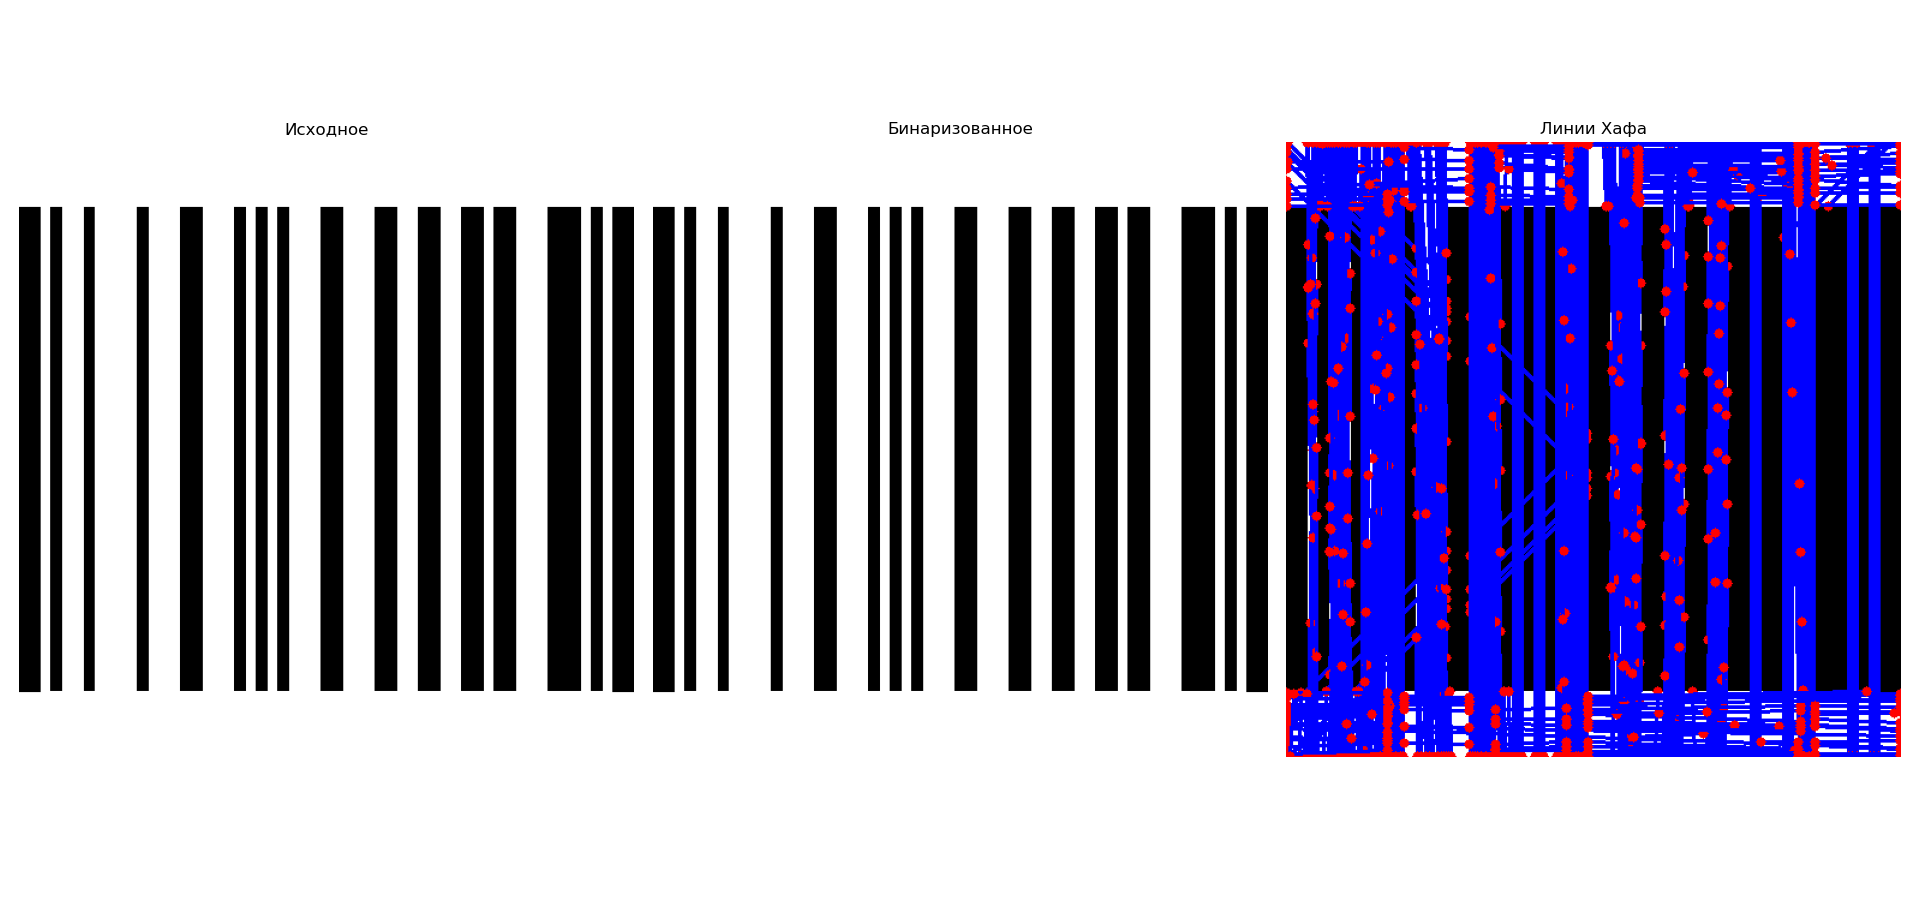
\includegraphics[width=1\textwidth]{Figure_22.png}
		\caption{Линии на изображении 2}
		\label{fig:lines}
	\end{figure}
	
	
	\begin{figure}[H]
		\centering
		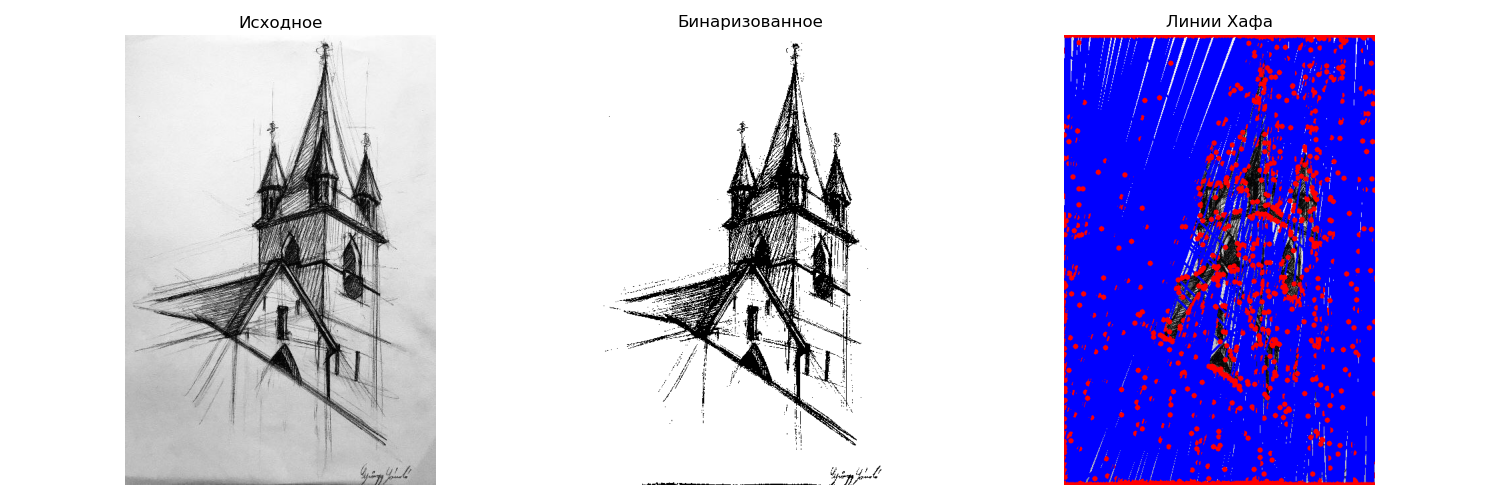
\includegraphics[width=1\textwidth]{Figure_32.png}
		\caption{Линии на изображении 3}
		\label{fig:lines}
	\end{figure}
	
	\subsection{Мини-вывод}
	
	
	Как показали эксперименты, Хаф хорошо ищет линии только после Кэнни. Без предварительного поиска границ алгоритм часто ошибается - находит лишнее и пропускает нужное. Лучше всего работает цепочка: сначала Кэнни выделяет контуры, потом Хаф ищет по ним линии. В итоге получаем: Хаф - мощный, но только в паре с Кэнни.
	
	
	
	\section{Task. Поиск окружностей}
	\subsection{Краткое условие}
	В этом задании нужно сделать поиск окружностей определенного радиуса и окружностей с радиусом в каком-то диапазоне значений. Применить перобразование Хафа как к исходному изображению, так и к изображению с диф. оператором.
	
	\subsubsection{С Собелем}
	
	Итак применю оператор Собеля, а затем преобразование Хафа к изображению, содержащее круги: отыщем круги в радиусе [15; 100].
	
	
		
	\begin{figure}[H]
		\centering
		
\includegraphics[width=1\textwidth]{Figure_10.png}
		\caption{Окружности на изображении 1}
		\label{fig:lines}
	\end{figure}
	
		
	\begin{figure}[H]
		\centering
		
\includegraphics[width=1\textwidth]{Figure_11.png}
		\caption{Окружности на изображении 2}
		\label{fig:lines}
	\end{figure}
	
		
	\begin{figure}[H]
		\centering
		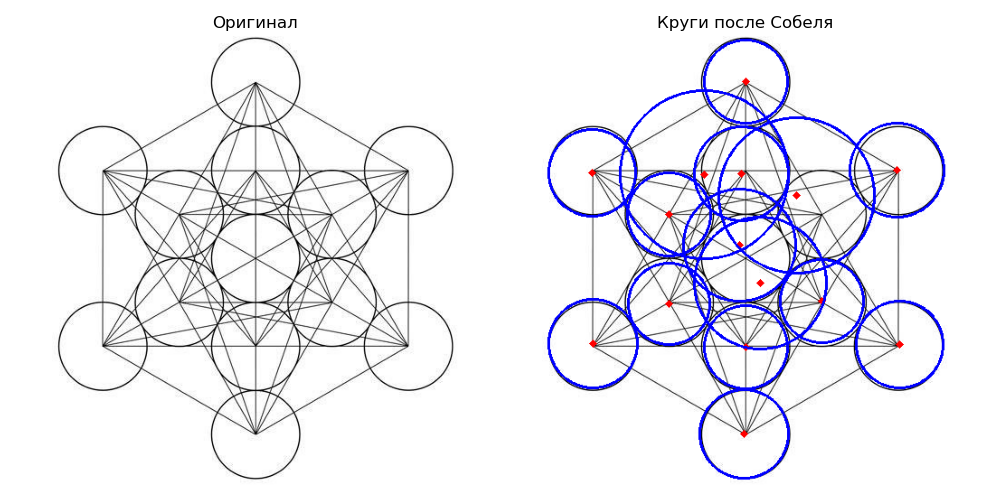
\includegraphics[width=1\textwidth]{Figure_13.png}
		\caption{Окружности на изображении 3}
		\label{fig:lines}
	\end{figure}
	
	
	\subsubsection{Без Собеля}
	Проделаю то же самое, но без преобразования Собеля:
	
	
	\begin{figure}[H]
		\centering
		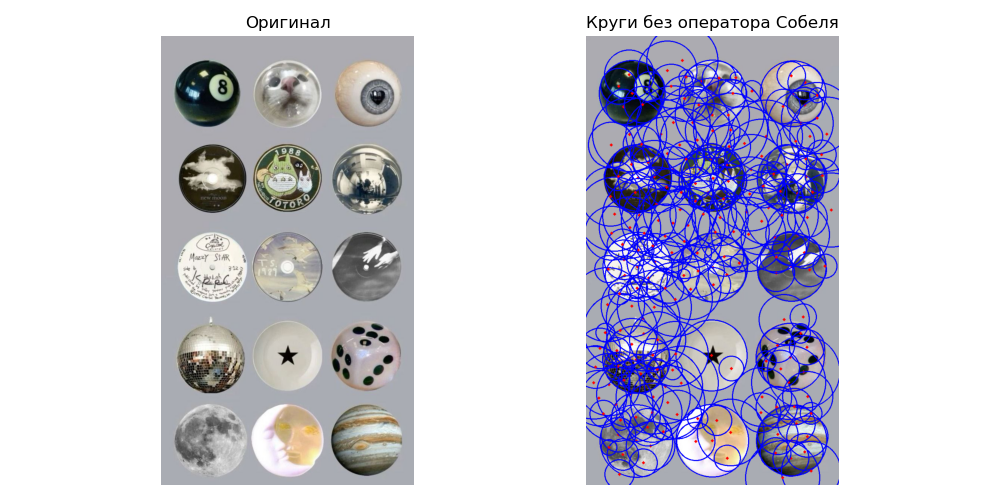
\includegraphics[width=1\textwidth]{Figure_20.png}
		\caption{Окружности на изображении 1}
		\label{fig:lines}
	\end{figure}
	
	
	\begin{figure}[H]
		\centering
		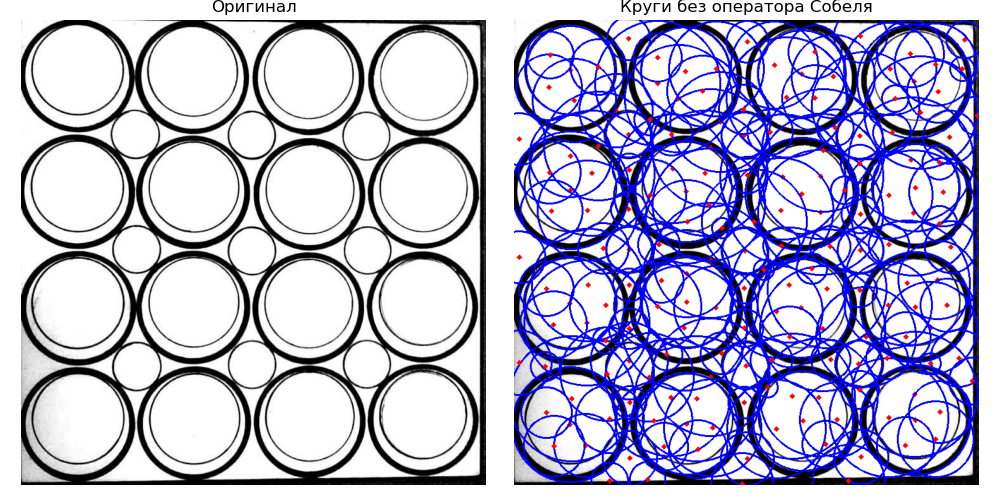
\includegraphics[width=1\textwidth]{Figure_30.png}
		\caption{Окружности на изображении 2}
		\label{fig:lines}
	\end{figure}
	
	
	\begin{figure}[H]
		\centering
		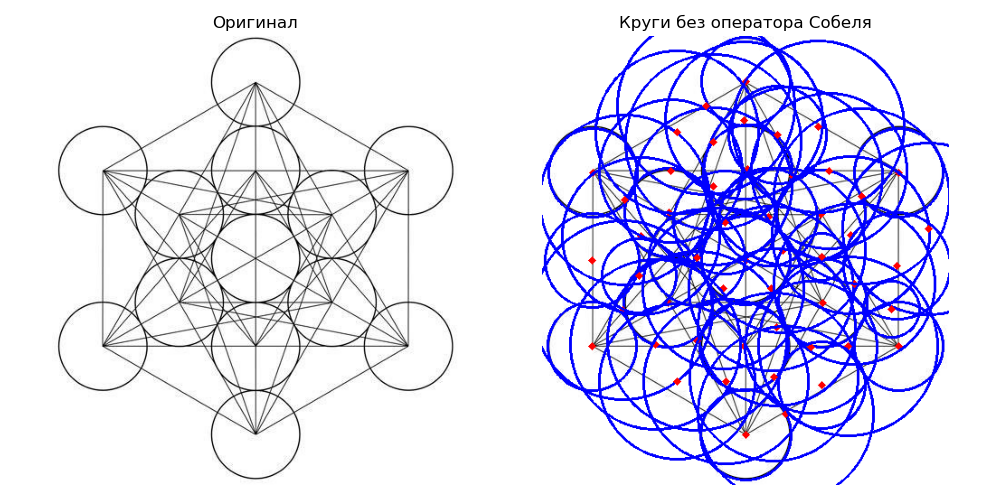
\includegraphics[width=1\textwidth]{Figure_40.png}
		\caption{Окружности на изображении 3}
		\label{fig:lines}
	\end{figure}
	
	\subsection{Мини-вывод}
	
	Как и в случае с линиями, преобразование Хафа даёт лучшие результаты после предварительной обработки изображения.  
	С использованием оператора Собеля круги распознаются точнее, контуры — чище, меньше шумов и ложных срабатываний.  
	Без оператора Собеля алгоритм работает менее стабильно: пропускает слабые круги или находит лишние.  
	
	
	
	
	\section{Ответы на вопросы}
	\begin{itemize}
		\item Какая идея лежит в основе преобразования Хафа?
		- Основная идея - идея о голосовании точек. То есть мы переводим фигуру из декартовой системы координат в параметрическую - получаем, что каждая точка из параметрической системы голосует кто она - то есть какому набору параметров фигуры она соответствует.
		
		\item Можно ли использовать преобразование Хафа для поиска
		произвольных контуров, которые невозможно описать анали-
		тически? - Да, но только в случае, если у нас будет эталонная фигура в пространстве параметров. Либо использовать обобщенное преобразование Хафа.
		
		\item Что такое рекуррентное и обобщенное преобразования Хафа? - Рекуррентное преобразование Хафа — упрощённый и быстрый метод, ищущий фигуры по выборке точек.
		
		Обобщённое преобразование Хафа — позволяет находить произвольные формы по шаблону, даже без уравнения.
		
		\item Какие бывают способы параметризации в преобразовании Хафа?-
		
		 Для прямых чаще всего используется полярная форма \( \rho = x \cos\theta + y \sin\theta \). Декартова форма \( y = kx + b \) менее надёжна, особенно при вертикальных прямых.
		
		Окружности описываются уравнением \( (x - a)^2 + (y - b)^2 = r^2 \), где параметры — центр \( (a, b) \) и радиус \( r \).
		
		Для произвольных контуров применяется обобщённое преобразование Хафа, использующее шаблон фигуры и таблицу направлений (R-table) вместо аналитического уравнения. 
	\end{itemize}
	
	\section{Примечание}
	\href{https://github.com/decadeos/ITMO/tree/master/2_course/texViz/lab5}{GitHub}
\end{document}